\documentclass[12pt,a4paper]{report}

% ---- Encoding & language ----------------------------------------------------
\usepackage[utf8]{inputenc}
\usepackage[T1]{fontenc}
\usepackage[english]{babel}

% ---- Page layout ------------------------------------------------------------
\usepackage[
  top=2.5cm, bottom=2.5cm,
  left=3cm,  right=2.5cm
]{geometry}

% ---- Typography -------------------------------------------------------------
\usepackage{lmodern}
\usepackage{microtype}
\usepackage{setspace}
\onehalfspacing

% ---- Math -------------------------------------------------------------------
\usepackage{amsmath}
\usepackage{amssymb}

% ---- Graphics & colour ------------------------------------------------------
\usepackage{graphicx}
\usepackage{xcolor}

% ---- TikZ (architecture diagram) -------------------------------------------
\usepackage{tikz}
\usetikzlibrary{shapes.geometric, arrows.meta, positioning, fit, backgrounds}

% ---- Tables -----------------------------------------------------------------
\usepackage{booktabs}
\usepackage{tabularx}
\usepackage{multirow}

% ---- Code listings ----------------------------------------------------------
\usepackage{listings}
\definecolor{codegray}{rgb}{0.95,0.95,0.95}
\definecolor{codeblue}{rgb}{0.0,0.0,0.6}
\lstset{
  backgroundcolor=\color{codegray},
  basicstyle=\ttfamily\small,
  keywordstyle=\color{codeblue}\bfseries,
  breaklines=true,
  frame=single,
  numbers=left,
  numberstyle=\tiny,
  captionpos=b,
  tabsize=4
}

% ---- Captions ---------------------------------------------------------------
\usepackage{caption}
\captionsetup{font=small, labelfont=bf}

% ---- Chapter / section title formatting -------------------------------------
% Reduces the default 50 pt top-of-chapter dead space and gives titles
% a clean, proportional size hierarchy (LARGE > large > normalsize).
\usepackage{titlesec}
\titleformat{\chapter}[hang]
  {\LARGE\bfseries}{\thechapter.}{0.6em}{}
\titlespacing*{\chapter}{0pt}{0pt}{1.4em}
\titleformat{\section}
  {\large\bfseries}{\thesection}{0.5em}{}
\titlespacing*{\section}{0pt}{1.2em}{0.6em}
\titleformat{\subsection}
  {\normalsize\bfseries}{\thesubsection}{0.5em}{}
\titlespacing*{\subsection}{0pt}{0.9em}{0.4em}

% ---- Headers and footers ----------------------------------------------------
\usepackage{fancyhdr}
\pagestyle{fancy}
\fancyhf{}
\fancyhead[L]{\small Tower Siege}
\fancyhead[R]{\small Technical Report -- 2026-I}
\fancyfoot[C]{\thepage}
\setlength{\headheight}{14pt}

% ---- References and links ---------------------------------------------------
\usepackage[
  backend=bibtex,
  style=ieee,
  sorting=none
]{biblatex}
\addbibresource{references.bib}

\usepackage[
  colorlinks=true,
  linkcolor=black,
  citecolor=blue,
  urlcolor=blue
]{hyperref}
\usepackage{bookmark}
\hypersetup{linktoc=all}

% ---- Metadata ---------------------------------------------------------------
\title{
  \vspace{-1cm}
  {\Large Universidad Distrital Francisco José de Caldas} \\[0.4cm]
  {\large Facultad de Ingeniería -- Computer Science I (2026-I)} \\[1.2cm]
  {\Huge\bfseries Tower Siege} \\[0.5cm]
  {\large A Grid-Based Tower-Defense Engine Demonstrating\\
   Linked Lists, Binary Search Trees, Greedy Placement,\\
   and Backtracking Pathfinding}
}
\author{
  Daniel Santiago Pérez Madera \\
  \textit{Codigo: 20231020203} \\[0.5cm]
  \texttt{dsperezm@udistrital.edu.co}
}
\date{June 2026}

% =============================================================================
\begin{document}
% =============================================================================

% ---- Title page -------------------------------------------------------------
\maketitle
\thispagestyle{empty}
\newpage

% ---- Abstract ---------------------------------------------------------------
\begin{abstract}
Tower-defense games provide a natural laboratory for evaluating how classical
algorithms behave under real-time constraints and adversarial inputs.
This report presents \textit{Tower Siege}, a two-layer system in which a C++ engine
manages game state using hand-implemented data structures---a singly linked list
for the active enemy wave and a Binary Search Tree for towers ordered by attack
power---while a Python layer runs a \textit{Greedy} tower-placement advisor and
a \textit{Backtracking} pathfinder, exchanging data exclusively through JSON files.
The project achieves a fully playable five-level game with two tower types, two
enemy types, real-time HUD feedback, and algorithm visualisation; however, a
systematic interaction between the Greedy scoring function and the Backtracking
DFS was identified in which the Greedy's castle-proximity bias progressively
narrows enemy corridors until the Backtracking's exponential search space causes
perceptible frame-rate degradation, an issue that is analysed in depth and whose
remediation is proposed as future work.
\end{abstract}
\newpage

% ---- Table of Contents ------------------------------------------------------
\cleardoublepage
\phantomsection
\tableofcontents
\cleardoublepage

% ---- List of Figures --------------------------------------------------------
\phantomsection
\listoffigures
\cleardoublepage

% =============================================================================
\phantomsection
\chapter{Introduction}
\label{ch:introduction}
% =============================================================================

Tower-defense games represent a category of real-time strategy in which the
player places static defensive units (towers) on a grid to prevent waves of
enemies from reaching a goal cell (the castle).
Beyond entertainment, this genre is a useful proxy for scheduling, resource
allocation, and pathfinding problems that appear in operations research and
algorithmic decision systems \cite{cormen2022algorithms}.

Prior solutions to in-game pathfinding range from simple breadth-first search
to $A^*$ with domain-specific heuristics \cite{hart1968astar}.
Tower-placement advice has been addressed through influence maps, potential
fields, and greedy heuristics that score candidate cells by their proximity
to high-traffic corridors.
The tension between placement strategies and pathfinding robustness---each tower
added reshapes the search space for path computation---motivates a direct study
of how these two components interact when integrated in the same game loop.

\textit{Tower Siege} was designed as an academic vehicle to implement and stress-test
four specific algorithmic and data-structural artefacts within a single coherent
application:

\begin{enumerate}
  \item A \textbf{singly linked list} (C++) maintaining the active enemy wave.
  \item A \textbf{Binary Search Tree} (C++) indexing towers by attack power.
  \item A \textbf{Greedy} heuristic (Python) recommending the best tile for the
        next tower.
  \item A \textbf{Backtracking DFS} (Python) computing the shortest obstacle-free
        path from each spawn point to the castle.
\end{enumerate}

The two computational layers communicate exclusively via JSON files on disk,
providing a clean inter-process boundary that mirrors real-world service
architectures \cite{python3json}.
The rest of this report is structured as follows: Chapter~\ref{ch:litreview}
surveys related literature; Chapter~\ref{ch:objectives} states the project goals;
Chapters~\ref{ch:scope}--\ref{ch:limitations} define scope, assumptions, and
limitations; Chapter~\ref{ch:methodology} describes design decisions and
architecture; Chapter~\ref{ch:implementation} presents the implemented system
and test results; Chapter~\ref{ch:discussion} analyses the identified
Greedy–Backtracking interaction bug; and Chapter~\ref{ch:conclusion} summarises
findings and proposes future work.

% =============================================================================
\cleardoublepage
\phantomsection
\chapter{Literature Review}
\label{ch:litreview}
% =============================================================================

\section{Greedy Algorithms}

A greedy algorithm builds a solution incrementally by always making the choice
that looks best at the current step without revisiting past decisions
\cite{cormen2022algorithms}.
The optimality guarantee holds when the problem exhibits the \textit{greedy-choice
property} and \textit{optimal substructure}; in general combinatorial settings
these conditions may not hold, and greedy produces an approximation rather than
an exact optimum \cite{cormen2022algorithms}.
In game-algorithm design, greedy heuristics are widely used for tower placement because they
run in $O(n \cdot m)$ time over an $n \times m$ grid and provide instantaneous
visual feedback, a requirement for real-time systems.
A common scoring approach combines enemy proximity, path frequency (influence
maps), and goal proximity; the choice of weights critically determines whether
the advisor steers the player toward effective or counterproductive placements
\cite{cormen2022algorithms}.

\section{Backtracking and Pathfinding}

Backtracking is a systematic DFS strategy that extends partial candidates and
prunes branches that cannot lead to a valid solution \cite{cormen2022algorithms}.
For grid pathfinding without heuristic guidance it is equivalent to exhaustive
DFS, with worst-case complexity $O(4^{n \cdot m})$ on an $n \times m$
grid \cite{cormen2022algorithms}.
Practical pathfinding in games typically uses $A^*$, which combines a
forward cost with an admissible heuristic to achieve $O(b^d)$ complexity
where $b$ is the branching factor and $d$ the optimal path depth
\cite{hart1968astar}.
Backtracking-based pathfinding is nevertheless instructive in academic settings
because it exposes how the search space grows with grid occupancy---a property
exploited in the bug analysis of Chapter~\ref{ch:discussion}.

\section{Data Structures in Game Engines}

Linked lists are the canonical container for dynamic entity sets where frequent
insertions and deletions occur at arbitrary positions, as in an enemy wave queue
\cite{cormen2022algorithms}.
Binary Search Trees provide $O(\log n)$ average-case search and sorted
traversal, making them appropriate for ordering towers by attack power to
display a real-time ranking \cite{cormen2022algorithms}.
Both structures are implemented here from scratch, following course requirements
that prohibit the use of STL equivalents such as \texttt{std::list} or
\texttt{std::map}.

% =============================================================================
\cleardoublepage
\phantomsection
\chapter{Objectives}
\label{ch:objectives}
% =============================================================================

\section{General Objective}

To design and implement a two-language, file-coupled tower-defense game that
demonstrates the application of hand-rolled data structures (linked list and BST)
and algorithmic strategies (Greedy and Backtracking) within a real-time,
interactive context.

\section{Specific Objectives}

\begin{enumerate}
  \item Implement a singly linked list in C++ to manage the active enemy wave,
        supporting $O(1)$ append, $O(n)$ removal by ID, and sequential
        traversal for advance and attack resolution.
  \item Implement an unbalanced BST in C++ to maintain towers ordered by
        attack power, supporting $O(h)$ insertion and $O(n)$ in-order traversal
        exported to the Python layer via JSON.
  \item Write a Greedy function in Python that scores every free cell of the
        grid and returns the cell with the highest incoming-threat score as a
        placement recommendation.
  \item Write a Backtracking DFS in Python that finds the shortest path from
        each spawn point to the castle cell, avoiding tower-occupied cells.
  \item Integrate both layers through a JSON file bridge so that all data
        exchange occurs through \texttt{input.json} (Python $\to$ C++) and
        \texttt{state.json} (C++ $\to$ Python).
  \item Build a Pygame UI that visualises algorithm decisions---highlighted
        greedy recommendation, drawn enemy paths, and BST-sorted tower
        list---and supports five game levels of increasing difficulty.
\end{enumerate}

% =============================================================================
\cleardoublepage
\phantomsection
\chapter{Scope}
\label{ch:scope}
% =============================================================================

\textit{Tower Siege} is scoped as a single-player, offline, grid-based
tower-defense game running on a local machine.
The project encompasses:

\begin{itemize}
  \item A C++ engine binary that reads one JSON command per invocation and
        writes one JSON state snapshot (stateless per-call model).
  \item A Python game loop (Pygame) that is the sole entry point
        (\texttt{game/ui/main.py}).
  \item Five levels with grids of $8 \times 8$ (levels 1--2) and
        $10 \times 10$ (levels 3--5), two tower types, two enemy types,
        and up to two spawn points.
  \item Algorithm visualisation: the greedy-recommended cell is highlighted
        in teal; enemy paths drawn as blue outlines; tower attack lines
        rendered each step; the BST order shown in the HUD panel.
\end{itemize}



% =============================================================================
\cleardoublepage
\phantomsection
\chapter{Assumptions}
\label{ch:assumptions}
% =============================================================================

\begin{enumerate}
  \item The C++ engine binary is compiled before the game is launched
        (\texttt{tower\_engine.exe} present at \texttt{engine/tower\_engine.exe}).
  \item Python 3.9 or later and Pygame 2.x are installed in the execution
        environment.
  \item The grid is always square (rows $=$ cols); non-square grids are
        undefined behaviour.
  \item Enemy HP values are always positive integers; the engine does not
        validate input ranges beyond assertions.
  \item Each enemy follows exactly one pre-computed path identified by its
        \texttt{path\_id} field; path recomputation happens only when the
        tower layout changes.
  \item Manhattan distance is the appropriate proximity metric for both
        tower attack range and greedy scoring, consistent with 4-directional
        grid movement.
  \item The castle cell is always at position $(\text{grid} - 1,\,
        \text{grid} - 1)$, and spawn points are always in row 0.
\end{enumerate}

% =============================================================================
\cleardoublepage
\phantomsection
\chapter{Limitations}
\label{ch:limitations}
% =============================================================================

\begin{enumerate}
  \item \textbf{Backtracking complexity.}
        The pathfinder uses exhaustive DFS with a pruning optimisation
        (branch pruned when the partial path plus the Manhattan lower bound
        to the goal already exceeds the current best).
        Worst-case complexity remains $O(4^{n \cdot m})$, which becomes
        perceptible on heavily occupied grids (see Chapter~\ref{ch:discussion}).
  \item \textbf{Unbalanced BST.}
        The BST does not implement rotations; degenerate insertion order
        (e.g., towers placed in strictly increasing attack-power order) reduces
        the tree to a linked list with $O(n)$ search.
  \item \textbf{Greedy sub-optimality.}
        The Greedy scoring function overweights castle proximity, causing
        systematic recommendations of near-castle cells that conflict with
        effective tower-defense strategy (detailed in
        Chapter~\ref{ch:discussion}).
  \item \textbf{Stateless engine.}
        The C++ engine reconstructs all data structures from the JSON payload
        on every invocation. For large grids or long waves this introduces
        unnecessary serialisation overhead.
  \item \textbf{No adaptive opponent.}
        Enemy routing is reactive (follows shortest available path) rather
        than adversarial; enemies do not adapt to tower placements beyond the
        path recomputation.
  \item \textbf{Single platform.}
        The engine binary path is hard-coded for Windows
        (\texttt{tower\_engine.exe}); a Makefile with a platform-detection
        variable would be required for Linux/macOS builds.
\end{enumerate}

% =============================================================================
\cleardoublepage
\phantomsection
\chapter{Methodology}
\label{ch:methodology}
% =============================================================================

\section{System Architecture}

Tower Siege uses a strict three-layer architecture mandated by the course
assignment.
The layers are decoupled by a file-based inter-process communication (IPC)
contract so that neither layer depends on the other's runtime.

\begin{figure}[ht]
\centering
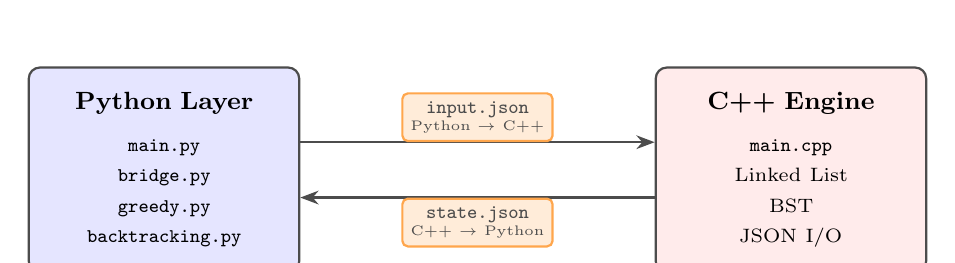
\begin{tikzpicture}[
  pybox/.style  = {draw=black!70, thick, rounded corners=4pt,
                   fill=blue!10, text width=3.2cm, align=center,
                   minimum height=2.6cm, font=\small},
  cppbox/.style = {draw=black!70, thick, rounded corners=4pt,
                   fill=red!8,   text width=3.2cm, align=center,
                   minimum height=2.6cm, font=\small},
  lbl/.style    = {rectangle, rounded corners=2pt, fill=orange!15,
                   draw=orange!70, font=\scriptsize,
                   inner sep=3pt, align=center},
  arr/.style    = {->, >=Stealth, thick, black!70}
]
\node[pybox] (py) {
  \textbf{Python Layer}\\[4pt]
  {\scriptsize\texttt{main.py}}\\
  {\scriptsize\texttt{bridge.py}}\\
  {\scriptsize\texttt{greedy.py}}\\
  {\scriptsize\texttt{backtracking.py}}
};
\node[cppbox, right=4.5cm of py] (cpp) {
  \textbf{C++ Engine}\\[4pt]
  {\scriptsize\texttt{main.cpp}}\\
  {\scriptsize Linked List}\\
  {\scriptsize BST}\\
  {\scriptsize JSON I/O}
};
\draw[arr] ([yshift=10pt]py.east)
  -- node[above, lbl]{\texttt{input.json}\\[-2pt]{\tiny Python $\to$ C++}}
  ([yshift=10pt]cpp.west);
\draw[arr] ([yshift=-10pt]cpp.west)
  -- node[below, lbl]{\texttt{state.json}\\[-2pt]{\tiny C++ $\to$ Python}}
  ([yshift=-10pt]py.east);
\end{tikzpicture}
\caption{Three-layer architecture of Tower Siege. The Python layer writes
  \texttt{input.json} (player command) and reads \texttt{state.json}
  (updated game state); the C++ engine does the inverse.}
\label{fig:architecture}
\end{figure}

Table~\ref{tab:layers} summarises each layer's language, files, and primary
responsibility.

\begin{table}[ht]
\centering
\caption{Layer responsibilities in Tower Siege.}
\label{tab:layers}
\begin{tabularx}{\linewidth}{lllX}
\toprule
\textbf{Layer} & \textbf{Language} & \textbf{Key files} & \textbf{Responsibility} \\
\midrule
Core Engine    & C++    & \texttt{main.cpp}, \texttt{linked\_list.cpp}, \texttt{tree.cpp}
               & Maintains enemy wave (linked list) and tower set (BST). Reads
                 \texttt{input.json}, writes \texttt{state.json}. \\
Algorithm      & Python & \texttt{greedy.py}, \texttt{backtracking.py}
               & Greedy tile scoring and backtracking pathfinding. Pure
                 functions; no I/O. \\
UI / Bridge    & Python & \texttt{main.py}, \texttt{bridge.py}
               & Pygame rendering, user input, level management, JSON exchange. \\
\bottomrule
\end{tabularx}
\end{table}

\section{Data Structures}

\subsection{Enemy Wave: Singly Linked List}

The active enemy wave is stored as a singly linked list (\texttt{EnemyList}
in \texttt{linked\_list.h}).
A dedicated \texttt{tail} pointer keeps append ($\texttt{ll\_push\_back}$)
at $O(1)$.
Removal of a dead enemy (\texttt{ll\_remove\_id}) requires an $O(n)$ scan
because the list is unordered by ID.
Each step, \texttt{ll\_advance} walks the list once and increments each enemy's
position along its pre-computed path by \texttt{speed} cells.

\subsection{Tower Registry: Binary Search Tree}

Towers are inserted into an unbalanced BST (\texttt{TowerTree} in
\texttt{BSTree.h}) keyed on \texttt{attack\_power}.
In-order traversal (\texttt{tt\_inorder}) yields towers sorted from weakest
to strongest; this sorted list is serialised into \texttt{state.json} and
displayed in the HUD panel to demonstrate the BST property visually.
Insertion is $O(h)$ where $h$ is tree height; with random attack-power values
$h \approx \log n$ on average.

\section{Algorithms}

\subsection{Greedy Tower Placement}

\texttt{greedy.recommend\_tile} iterates over every free cell of the grid and
computes a scalar threat score:

\[
  S(r,c) = \sum_{\substack{e \in \text{enemies} \\ d_e \le 7}}
             (8 - d_e)\,\frac{e.\text{hp}}{100}
           \;+\; \max\!\bigl(0,\,8 - d_\text{castle}\bigr) \cdot 1.5
\]

where $d_e = |r - e_r| + |c - e_c|$ is the Manhattan distance to enemy $e$
and $d_\text{castle}$ is the Manhattan distance to the castle.
The cell with the highest score is returned as the recommended placement and
highlighted in teal on the grid.
Complexity is $O(n \cdot m \cdot |\text{enemies}|)$.

\subsection{Backtracking Pathfinding}

\texttt{backtracking.find\_path} performs DFS from each spawn point to the
castle cell, exploring the four cardinal neighbours and pruning branches
whenever the partial path length plus the Manhattan lower bound to the goal
already meets or exceeds the current best-found path length.
The function returns the shortest path (minimum number of steps) or an
empty list if no path exists.
\texttt{game/ui/main.py} also uses this function in
\texttt{placing\_blocks\_path} to prevent the player from sealing off all
enemy routes before placing a new tower.

\section{JSON Communication Contract}

The engine reads \texttt{data/input.json} and writes \texttt{data/state.json}
on each invocation (Table~\ref{tab:json}).
The C++ engine implements its own JSON serialiser/parser using only the
standard library, as required by course constraints---the
\texttt{nlohmann/json} library \cite{nlohmann2024json} was considered but
excluded because external C++ dependencies are forbidden by the assignment.

\begin{table}[ht]
\centering
\caption{Top-level fields in the JSON contract.}
\label{tab:json}
\begin{tabularx}{\linewidth}{llX}
\toprule
\textbf{File} & \textbf{Field} & \textbf{Description} \\
\midrule
\texttt{input.json}
  & \texttt{command}    & One of \texttt{"init"}, \texttt{"step"},
                          \texttt{"place\_tower"}, \texttt{"remove\_tower"} \\
  & \texttt{grid}       & \texttt{\{rows, cols\}} -- grid dimensions \\
  & \texttt{castle}     & \texttt{\{row, col\}} -- castle position \\
  & \texttt{castle\_hp} & Current castle hit points \\
  & \texttt{towers}     & Array of tower objects \\
  & \texttt{enemies}    & Array of enemy objects \\
  & \texttt{paths}      & Array of paths (one per spawn); each path is an
                          array of \texttt{\{row,col\}} waypoints \\
\midrule
\texttt{state.json}
  & \texttt{castle\_hp}       & Updated castle HP after the step \\
  & \texttt{towers\_by\_power}& Towers in ascending attack-power order (BST in-order) \\
  & \texttt{enemies}          & Updated enemy array \\
  & \texttt{events}           & Events emitted: \texttt{tower\_attack},
                                \texttt{enemy\_killed}, \texttt{castle\_damaged},
                                \texttt{wave\_clear} \\
\bottomrule
\end{tabularx}
\end{table}

\section{Level Design}

Five levels of escalating difficulty are defined in \texttt{levels.py}
(Table~\ref{tab:levels}).
Levels 1--2 use an $8 \times 8$ grid; levels 3--5 use $10 \times 10$.
Level~5 introduces a second spawn point at $(0, 9)$, requiring the
Backtracking to compute two independent paths simultaneously.

\begin{table}[ht]
\centering
\caption{Level configuration summary.}
\label{tab:levels}
\begin{tabular}{ccccccc}
\toprule
\textbf{Level} & \textbf{Grid} & \textbf{Enemies} & \textbf{Spawn~ms}
  & \textbf{Tower budget} & \textbf{Heavy?} & \textbf{Spawns} \\
\midrule
1 &  $8\!\times\!8$  &  5 & 4000 & 4 & No  & 1 \\
2 &  $8\!\times\!8$  &  6 & 3500 & 4 & No  & 1 \\
3 & $10\!\times\!10$ &  7 & 3500 & 5 & Yes & 1 \\
4 & $10\!\times\!10$ &  8 & 3000 & 5 & Yes & 1 \\
5 & $10\!\times\!10$ & 10 & 3000 & 6 & Yes & 2 \\
\bottomrule
\end{tabular}
\end{table}

% =============================================================================
\cleardoublepage
\phantomsection
\chapter{Implementation \& Results}
\label{ch:implementation}
% =============================================================================

\section{Development Environment}

The project was developed on Windows~11 using:
\begin{itemize}
  \item \textbf{C++17} compiled with \texttt{g++ -std=c++17 -O2} (MinGW-w64).
  \item \textbf{Python 3.12} with \textbf{Pygame 2.x} \cite{pygame2024docs}.
  \item No third-party C++ libraries; JSON parsing implemented by hand in
        \texttt{engine/JsonIO.cpp}.
\end{itemize}

\section{C++ Engine}

The engine (\texttt{engine/main.cpp}) executes the following flow on each
invocation:

\begin{enumerate}
  \item Parse \texttt{input.json} with \texttt{read\_input()}.
  \item Rebuild the \texttt{EnemyList} and \texttt{TowerTree} from the
        deserialized vectors.
  \item Apply the requested command.
        For a \texttt{"step"} command: advance all enemies one tick
        (\texttt{ll\_advance}), resolve tower attacks
        (\texttt{apply\_tower\_attacks}), resolve castle damage
        (\texttt{resolve\_castle\_damage}).
        Other commands echo state without modifications.
  \item Serialise the resulting \texttt{GameState} to \texttt{state.json}
        with \texttt{write\_state()}.
\end{enumerate}

Tower attacks are resolved from weakest to strongest (in-order BST traversal);
each tower targets the \textit{nearest} alive enemy within its Manhattan
radius.

\section{Python Layer}

The Python layer consists of four modules:
\begin{itemize}
  \item \texttt{bridge.py} -- writes \texttt{input.json}, launches the engine
        via \texttt{subprocess.run}, reads \texttt{state.json}.
  \item \texttt{greedy.py} -- pure function; returns recommended cell.
  \item \texttt{backtracking.py} -- pure function; returns path as list of
        waypoints.
  \item \texttt{levels.py} -- pure data; defines LEVELS, TOWER\_TYPES, and
        ENEMY\_TYPES.
\end{itemize}

The Pygame UI (\texttt{main.py}) runs at 30~FPS with a 1-second engine step
interval and a per-level configurable enemy spawn interval.

\section{Screenshots}

Figure~\ref{fig:gameplay} shows a running game session with the Greedy
recommendation and Backtracking path both visible.
Figure~\ref{fig:hud} shows the HUD panel where the BST in-order listing
is rendered in real time.

\begin{figure}[ht]
  \centering
  \includegraphics[width=0.92\linewidth]{image/gameplay_level3.png}
  \caption{Gameplay screenshot. The teal cell is the Greedy-recommended
    placement; blue outlines trace the Backtracking path from the spawn
    point to the castle. The diamond outline around a tower shows its
    Manhattan attack radius.}
  \label{fig:gameplay}
\end{figure}

\begin{figure}[ht]
  \centering
  \includegraphics[width=0.92\linewidth]{image/hud_bst.png}
  \caption{HUD panel. The ``BST by power'' list displays towers in
    ascending \texttt{attack\_power} order, directly demonstrating the
    BST in-order traversal property at runtime regardless of placement
    order.}
  \label{fig:hud}
\end{figure}

\section{Validation Results}

Due to the interactive nature of the game the test strategy was divided into
three phases:

\paragraph{Unit validation (informal).}
Each module was exercised in isolation before integration.
\texttt{greedy.py} was called with hand-crafted enemy sets to verify the
scoring formula; \texttt{backtracking.py} was run against small grids with
known shortest paths.
The C++ engine was invoked directly with manually authored JSON files to
confirm list/BST operations and event emission.

\paragraph{Integration validation.}
The full pipeline (Python writes \texttt{input.json} $\to$ engine runs $\to$
Python reads \texttt{state.json}) was verified by playing all five levels to
completion.
Enemy HP decremented correctly across steps, the BST in-order listing matched
manual inspection, and \texttt{wave\_clear} events triggered level transitions.

\paragraph{Acceptance validation.}
A session of each level was played under the intended use-case (player follows
the greedy hint) and under an adversarial use-case (player ignores the hint and
places towers sub-optimally).
Both sessions terminated correctly with a win or lose outcome and no Python
exceptions.

Table~\ref{tab:tests} summarises the validation cases.

\begin{table}[ht]
\centering
\caption{Summary of validation cases.}
\label{tab:tests}
\begin{tabularx}{\linewidth}{llX}
\toprule
\textbf{Category} & \textbf{Case} & \textbf{Expected / Observed} \\
\midrule
Unit   & Greedy with no enemies    & Returns $(0,0)$ (default; no enemies to score) -- \textbf{Pass} \\
Unit   & Backtracking, open grid   & Shortest path length $= (r-1)+(c-1)$ for goal $(r,c)$ -- \textbf{Pass} \\
Unit   & Backtracking, fully blocked & Returns empty list -- \textbf{Pass} \\
Unit   & BST in-order traversal    & Towers emitted in ascending attack\_power order -- \textbf{Pass} \\
Unit   & Linked list advance       & Enemy position increments by \texttt{speed} cells each step -- \textbf{Pass} \\
Integ. & Engine step (no towers)   & Enemy advances, no events; castle\_hp unchanged -- \textbf{Pass} \\
Integ. & Tower kills enemy         & \texttt{enemy\_killed} event emitted; enemy removed from list -- \textbf{Pass} \\
Integ. & Enemy reaches castle      & \texttt{castle\_damaged} event; castle\_hp decreases by 10 -- \textbf{Pass} \\
Accept.& Level 1 win               & 5 kills, castle HP $> 0$ -- \textbf{Pass} \\
Accept.& Castle falls (level 2)    & \texttt{lost} phase shown; press R resets -- \textbf{Pass} \\
Accept.& Path-block prevention     & Tower that would seal spawn rejected by \texttt{placing\_blocks\_path} -- \textbf{Pass} \\
\bottomrule
\end{tabularx}
\end{table}

% =============================================================================
\cleardoublepage
\phantomsection
\chapter{Discussion}
\label{ch:discussion}
% =============================================================================

\section{Greedy–Backtracking Interaction Bug}

The most significant observed issue in Tower Siege arises from the interaction
between the Greedy scoring function and the Backtracking pathfinder.
This section analyses the root cause, the trigger conditions, and the
measurable effect, and proposes two remediation strategies.

\subsection{Root Cause: Castle-Proximity Bias in Greedy}

The Greedy score for cell $(r, c)$ includes the term

\[
  \max\!\bigl(0,\,8 - d_\text{castle}\bigr) \cdot 1.5
\]

where $d_\text{castle} = |r - r_\text{castle}| + |c - c_\text{castle}|$.
Because this term is multiplied by a weight of $1.5$ and applies to
\textit{every} cell regardless of enemy proximity, cells adjacent to the
castle cell receive a bonus of up to $7 \times 1.5 = 10.5$ score units.
On an empty board with few enemies, or when enemies are far from the castle,
this proximity bonus dominates the threat sum and the Greedy consistently
recommends cells in the bottom-right quadrant---the neighbourhood of the
castle.

\subsection{Pathfinder Exposure}

As the player follows the Greedy recommendations, the bottom-right area
becomes progressively filled with towers.
The Backtracking DFS must then route enemies through the remaining free cells,
which form an increasingly narrow corridor.
Although the pruning optimisation

\[
  \text{len}(\text{path}) + d_\text{Manhattan}(\text{current, goal}) \ge \text{len}(\text{best})
  \implies \text{prune}
\]

eliminates many branches once a first path is found, the \textit{first}
solution may require exploring a large fraction of the search space when the
best path is long and convoluted.
In the worst case (a maze-like corridor of length $L$ through an $n \times m$
grid), the DFS visits $O(4^L)$ states before finding the first path.

Furthermore, \texttt{placing\_blocks\_path}---the guard that prevents the
player from sealing all routes---calls \texttt{find\_path} on every attempted
tower placement.
As the grid fills, this validation itself becomes slow, amplifying the
perceptible pause before each tower is accepted or rejected.

\subsection{Observable Symptom}

On a $10 \times 10$ grid in level~5 with several towers placed near the
castle (as recommended by Greedy), the following behaviour occurs:
\begin{enumerate}
  \item The player clicks a cell adjacent to an existing tower cluster.
  \item \texttt{placing\_blocks\_path} invokes \texttt{find\_path} for each
        of the two spawn points.
  \item With a narrow remaining corridor, each DFS explores a large number of
        candidate paths before finding the shortest.
  \item The Pygame event loop is blocked for the duration of the DFS
        (Python is single-threaded).
  \item The game appears to \textbf{freeze} for several seconds.
\end{enumerate}
If all routes to the castle happen to be blocked despite the guard (e.g.
by a race condition between the spawn timing and the placement check),
\texttt{find\_path} returns an empty list, the engine receives an empty paths
array, and enemies remain stationary---another freeze condition.

\subsection{Proposed Remediations}

Two remediation strategies are identified:

\paragraph{Short-term: re-weight the Greedy scoring function.}
Reducing the castle-proximity weight from $1.5$ to $0.3$--$0.5$ would shift
recommendations toward cells along the middle of the likely enemy routes
rather than near the castle.
A proper influence map---precomputed by flooding the grid from each spawn
point---would provide path-frequency data as a stronger signal than raw
castle distance.

\paragraph{Long-term: replace Backtracking with $A^*$.}
Using $A^*$ with the Manhattan heuristic would reduce worst-case path
computation from $O(4^L)$ to $O(b^d)$ with $b \approx 2.5$ on average
for grid graphs \cite{hart1968astar}.
Because $A^*$ is guaranteed to find the shortest path without exhaustive
exploration, the \texttt{placing\_blocks\_path} guard would run in
milliseconds rather than seconds even on highly occupied grids.
This change is confined to \texttt{backtracking.py} and would not require
any modification to the C++ engine or the JSON contract.

\section{Data Structure Performance}

The unbalanced BST performed adequately during testing because tower attack
powers take only two distinct values (15 for base towers, 40 for heavy towers).
With only two distinct key values the tree height is bounded by 2, so all
operations are effectively $O(1)$.
A future variant with continuous attack-power upgrades would expose the
absence of balancing and benefit from AVL or Red-Black rotations
\cite{cormen2022algorithms}.

The linked list showed constant-time append and acceptably linear removal for
wave sizes up to 10 enemies, consistent with the $O(n)$ theoretical bound.

% =============================================================================
\cleardoublepage
\phantomsection
\chapter{Conclusion}
\label{ch:conclusion}
% =============================================================================

Tower Siege successfully demonstrates the integration of four classical
computer-science artefacts---a singly linked list, a Binary Search Tree,
a Greedy heuristic, and a Backtracking DFS---within a playable, five-level
tower-defense game.
The strict separation between the C++ engine and the Python algorithm/UI
layers, enforced through a JSON file contract, proved effective: each layer
can be tested in isolation, and the contract acts as a self-documenting
interface specification.

The main engineering finding is that algorithm interactions must be analysed
holistically, not in isolation.
Individually, the Greedy function and the Backtracking pathfinder behave
correctly; together, the Greedy's castle-proximity bias progressively exposes
the Backtracking's exponential worst-case complexity.
This interaction is a concrete instance of the general principle that locally
optimal decisions (Greedy placement near the castle) can globally degrade
system performance (Backtracking freeze).

Future work should address three open points:
\begin{enumerate}
  \item Re-weight or replace the Greedy scoring function using a path-frequency
        influence map to bias recommendations toward high-traffic corridors.
  \item Replace the Backtracking DFS with $A^*$ to eliminate the exponential
        worst case in path computation and placement validation.
  \item Implement AVL balancing in the BST to guarantee $O(\log n)$
        performance when attack-power values span a wide range.
\end{enumerate}

% =============================================================================
% References
% =============================================================================
\printbibliography[heading=bibintoc, title={References}]

% =============================================================================
\end{document}
